% === Begin Label Data ===
% ID: 837
% 难度星级: 
% 标签: 
% 备注: 
% 组卷引用次数: 0
% === End  Label Data ===

\begin{problem}{2013}{G}{浙江卷}{16}{解三角形}
$\triangle ABC$ 中，$\angle C=90^\circ$，$M$ 是 $BC$ 的中点，若 $\sin\angle BAM=\dfrac{1}{3}$，则 $\sin\angle BAC=$\underline{\hspace{4em}}.
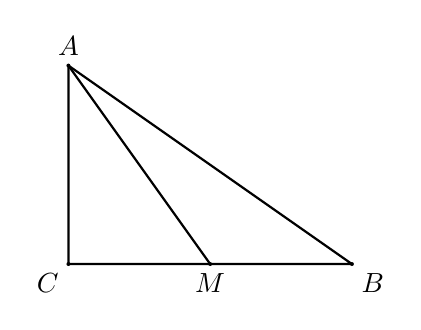
\begin{tikzpicture}[line cap=round,line join=round,scale=0.6]
% right triangle at C, with M midpoint of BC, draw AM and AB

\coordinate (C) at (0,0);
\coordinate (B) at (6,0);
\coordinate (M) at (3,0);
\coordinate (A) at (0,4.2);

% triangle edges
\draw[thick] (A)--(C)--(B)--cycle;

% median-like segment AM
\draw[thick] (A)--(M);

% points and labels
\fill (A) circle (1.2pt) node[above] {$A$};
\fill (B) circle (1.2pt) node[below right] {$B$};
\fill (C) circle (1.2pt) node[below left] {$C$};
\fill (M) circle (1.2pt) node[below] {$M$};

\end{tikzpicture}
\end{problem}

\begin{answer}
$\dfrac{\sqrt{6}}{3}$
\end{answer}

\begin{solutions}
设 $\angle BAC=\alpha$，$\angle MAC=\beta$，$\angle BAM=\gamma$，则 $\tan\gamma=\dfrac{\dfrac{1}{3}}{\sqrt{1-\left(\dfrac{1}{3}\right)^2}}=\dfrac{\sqrt{2}}{4}$

由 $M$ 是 $BC$ 中点可知 $\tan\alpha=2\tan\beta$：

$\tan\alpha=2\tan\beta=2\tan(\alpha-\gamma)=\dfrac{2\tan\alpha-2\tan\gamma}{1+\tan\alpha\tan\gamma}=\dfrac{2\tan\alpha-\dfrac{\sqrt{2}}{2}}{1+\dfrac{\sqrt{2}}{4}\tan\alpha}$

解得 $\tan\alpha=\sqrt{2}$，进而 $\sin\alpha=\dfrac{\sqrt{6}}{3}$.
\end{solutions}